\documentclass[11pt]{article}
\usepackage[a4paper,margin=25mm]{geometry}
\usepackage[T1]{fontenc}
\usepackage{lmodern,amsmath,amssymb,amsthm,mathtools,booktabs,longtable,array}
\usepackage[dvipsnames]{xcolor}
\usepackage{graphicx,microtype,fancyhdr}
\usepackage[colorlinks=true,linkcolor=MidnightBlue,urlcolor=MidnightBlue,citecolor=MidnightBlue]{hyperref}
\newtheorem{theorem}{Theorem}
\newtheorem{lemma}[theorem]{Lemma}
\newcommand{\id}{\mathrm{id}}
\newcommand{\Tr}{\operatorname{Tr}}
\newcommand{\supp}{\operatorname{supp}}
\newcommand{\norm}[1]{\left\lVert #1\right\rVert}
\newcommand{\cL}{\mathcal L}
\newcommand{\cD}{\mathcal D}
\newcommand{\cC}{\mathcal C}
\newcommand{\cE}{\mathcal E}
\newcommand{\ee}{\mathrm e}
\pagestyle{fancy}\fancyhf{}
\fancyhead[L]{\small Output-only experiments and deferred calibration}
\fancyhead[R]{\small Astra scientific construction}
\fancyfoot[C]{\thepage}\setlength{\headheight}{14pt}
\title{\textbf{Output-only experiments and recovery\\before Hamiltonian calibration}}
\author{Astra research construction}\date{5 November 2026}
\begin{document}
\setlength{\emergencystretch}{3em}
\hypersetup{pageanchor=false}
\begin{titlepage}\maketitle\thispagestyle{empty}\vspace{8mm}
\noindent\textbf{Completed capability.}
Capture a first arbitrary, unencoded many-body quantum input through calibrated coherent noise outputs; learn its previously unknown local Hamiltonian from later outputs of the same source; then recover that original input and its external reference correlations. No later copy of the original input and no direct source preparation, control or readout is required.

\vspace{5mm}\noindent\textbf{New construction.}
Retained replacement-state purifiers supply local process probes. A signed emission record has a fixed-order mixed derivative equal to one Hamiltonian coefficient. Finite interpolation acquires that derivative with all failed attempts counted. An adaptive-decoder lemma permits calibration records to remain correlated with the archived quantum state. A bounded-neighborhood companion removes equilibration waits.

\vspace{5mm}\noindent\textbf{Governing scope.}
Actual pure, calibrated, losslessly collected Weyl ports, a complete local Hamiltonian class, stationarity, protected receiver memory and paid finite controls are substantive premises. The known-Hamiltonian continuous reader is the accepted P1 operation at revision \texttt{324acb589443002bf8d529cc15e160129c5e36d2}. Calibration works at every \(r>0\); generic first-payload recovery uses P1's sufficient condition \(r>\beta_0\).

\vspace{5mm}\noindent\textbf{Limits.}
No competitive laboratory implementation, fixed-hardware asymptotic reader, arbitrary unknown-port calibration, natural-system completeness or historical priority is established. Explicit conservative constants are extremely large. The completed consequence is a finite polynomial-resource capability theorem.
\vfill
\noindent The previous full classical-feedback acquisition theorem, separate global-budget result, matched fixed-order parity/GHZ law, finite-slew and meter calibrations, and thermal-effusion operation are preserved unchanged.
\end{titlepage}\hypersetup{pageanchor=true}
\tableofcontents\newpage

\section{Question, consequence and strongest alternatives}
The next question is whether knowing the apparatus dynamics \emph{before the first specimen arrives} is essential for quantum acquisition. In the specified interface, it is not. The receiver can acquire an undecoded quantum record, use future emissions to learn the dynamics, and decode the first record later. The target is the original quantum channel, including arbitrary references; a classical state estimate would not achieve it.

The operative principle is that a pure replacement channel exports two resources: the preceding source state and a purifier of its replacement. The first carries the payload; the second makes subsequent dynamics experimentally accessible. Discarding the second can erase every stationary Hamiltonian-identification signal in the first.

Three results are separate: a heralded local process oracle at any \(r>0\); an unconditioned correlation experiment learning a fixed-locality Hamiltonian class with inverse-square accuracy dependence up to logarithms; and a first-payload recovery corollary removing prior knowledge of \(H\). The finite receiver implementation is inherited from P1, with its growing demands charged.

Stationary-output identification is established: Gu\c{t}\u{a}--Kiukas identify ergodic quantum Markov dynamics up to phase and unitary coordinate changes, and derive local asymptotic normality \cite{guta}. Their general result does not itself give this uniform many-body, local-hardware, first-payload recovery construction. No new claim that outputs contain dynamical information is made.

Efficient derivative-based Hamiltonian and Lindbladian learning is established \cite{franca}; high-temperature Gibbs and real-time learning have strong sample and computational guarantees \cite{haah}. Pseudo-Choi methods can be substantially more efficient when their controlled forward/inverse evolution access is supplied \cite{castaneda}. Here the required correlation is physically acquired from a source accessible only through its outgoing calibrated fields.

Gong et al.'s October 2026 \emph{Out-of-control Hamiltonian Learning} reconstructs generic two-local models using uniform source preparation and measurements, and specified lattice models using computational-basis preparation and measurements \cite{gong}. Those are restrictive but still direct source interfaces. This construction supplies its probes through outgoing purifiers.

Liu et al.'s October 2026 local-probe construction learns bounded-degree two-body models with one measurable qubit, fast single-qubit source controls and a reference backbone, achieving Heisenberg precision scaling \cite{liu}. That is a strong alternative when those controls exist; no precision or runtime superiority over it is claimed. Navascu\'es constructs probabilistic resetting of uncontrolled systems with interacting probes and unknown Hamiltonians \cite{navascues}. Its access and generic-success promises differ; its general \(O(d_S^3)\)-probe construction is exponential in source qubit count.

Relative to accepted P1 \cite{p1}, the achieved new consequence is precise: \(H\) need not be supplied before collecting the first arbitrary payload. The contribution is the finite polynomial local acquisition and uniform channel composition, beyond a qualitative combination of generic output identifiability and a known-model decoder. Port axes, phases, rates and coherent delivery remain supplied. No separation from every possible same-output-access calibration algorithm, or historical novelty of the complete composition, has been established.

\section{Premises and the inherited acquisition primitive}
Let \(S\) contain \(n\) qubits, \(d=2^n\), with static Hamiltonian
\[
H=\sum_{a=1}^{M}\theta_aP_a,\quad |\supp P_a|\le k,\quad B_H\ge\sum_a|\theta_a|.
\]
The distinct nonidentity Pauli list is complete and known, with unknown coefficients. Taking all weight-at-most-\(k\) Paulis allows unknown support and gives \(M=O(n^k)\) at fixed \(k\). An identity term is irrelevant and unidentifiable. Define
\[
\cL_H(\rho)=-i[H,\rho]+r\sum_i(\cE_i(\rho)-\rho),\quad
\cE_i(\rho)=I_i/2\otimes\Tr_i\rho,\quad \Lambda=2B_H+2nr.
\]
Known nonidentity Weyl ports \(L_{i,\mu}=\sqrt r\,W_{i,\mu}/2\), pure vacuum inputs and actual lossless coherent output access are premises. They fix the physical Pauli frame. The physical photon rate \(R_{\rm ph}=3nr/4\) differs from the synthetic reset rate \(r\).

P1's finite-bin receiver supplies
\begin{equation}
V|\psi\rangle=\sqrt{1-p}\,|\psi\rangle_S|\emptyset\rangle
+\sqrt p\,|\Phi_2\rangle_{S,A}|\psi\rangle_B,\qquad p=1-\ee^{-r\Delta}.
\label{eq:primitive}
\end{equation}
Flags are orthogonal with input-independent probabilities. \(B\) contains the old state with all references; \(A\) purifies the fresh source. This receiver operation grants no source SWAP or controlled source reset. P1 already uses replacement purifiers in its diagonal companion; the primitive itself is inherited.

For supplied \(\beta(H)\le\beta_0<r\), where
\[
\beta(H)=\max_i\sum_{X\ni i}(|X|-1)\operatorname{osc}(h_X),\qquad \kappa_0=r-\beta_0,
\]
P1's reverse-history receiver obeys
\begin{equation}
\norm{\overline{\cD}_{H,T}\cC_{H,T}-\id}_\diamond\le2\sqrt{n\ee^{-\kappa_0T}}.
\label{eq:p1}
\end{equation}
Its collector needs known noise parameters and norm bounds, not the coefficients of \(H\). Only the eventual inverse-history decoder needs those coefficients. This distinction permits deferred calibration.

\section{A local process oracle from outgoing fields}
Temporarily start the source in \(I/d\). For \(X\) of size \(b\), retain each site's \emph{last} replacement purifier in a front window of width \(w\). Let the source evolve for \(\tau\), discarding intervening output. In a back window of width \(w\), retain the \emph{first} export from each site of \(X\). Accept when all required resets occur; its ideal probability is \((1-\ee^{-rw})^{2b}\).

If \(H\) is omitted only during the two windows, the accepted state is the normalized Choi state of
\[
\mathcal T_X^\tau(\rho_X)=\Tr_{\bar X}\ee^{\tau\cL_H}
(\rho_X\otimes I_{\bar X}/2^{n-b}).
\]
Restoring \(H\) during those windows changes the state by at most \(4B_Hw\) on every ideal reset record: telescope unitary segments of total duration \(2w\) through normalized conditional CPTP reset maps. No inverse clock probability multiplies this timing bound.

This gives local process tomography. Bell-projecting a receiver input with the retained purifier, accepting the identity Bell outcome, adds success probability \(4^{-b}\) and yields a chosen-input query to \(\mathcal T_X^\tau\), reference-uniformly. Failed queries consume the input; there is no repeat-until-success claim on one unknown state. Choi tomography and teleportation are established machinery; the construction is their acquisition from these actual ports.

The \(4B_Hw\) estimate is a state bound. Writing \(\xi=4B_Hw<4^{-b}\),
a conservative input/reference-uniform bound after the Bell postselection is
\(2\xi/(4^{-b}-\xi)\). An unconditional physical instrument error must also
be divided by a lower bound on the full accepted probability. Thus window
width, clock successes and Bell conditioning are all paid. The main learning
construction below retains failures as outcomes and needs no such division.

\section{The signed-output identity}
For candidate \(P=P_a\), choose \(i\in\supp P\) and single-site Pauli \(Q_i\)
anticommuting with \(P_i\). Put \(R_P=iPQ_i\), a signed Hermitian Pauli,
\(b=|\supp P|\), and \(s=b+1\). Use the front window on \(\supp P\), but only
one back export at \(i\). Measure \(R_P^T\) on the front purifiers and \(Q_i\)
on that export. The raw result is their signed product on success and zero
otherwise:
\[
Y\in\{-1,0,1\},\quad f_P(w,\tau)=\mathbb EY,\quad
\mathbb EY^2=(1-\ee^{-rw})^s.
\]
Every attempted window is counted. Purifiers can instead be measured immediately
in their fixed Pauli bases, retaining only the last classical outcome per site.
Deferred measurement gives the same law, so this calibration needs no long-lived
entangled register.

\begin{theorem}[Acquired mixed derivative]
For source start \(I/d\),
\begin{equation}
\boxed{\partial_w^{\,s}\partial_\tau f_P(0,0)=2s!\,r^s\theta_P.}
\label{eq:identity}
\end{equation}
\end{theorem}
\begin{proof}
Success needs \(b\) selected front resets and one selected back reset. At order
\(w^s\), these are the only window insertions. Any Hamiltonian action, extra reset
or waiting expansion there adds a power of \(w\). The front resets create Bell
pairs and the back reset exports the required output, so
\[
[w^s]f_P(w,\tau)
=r^s2^{-n}\Tr[R_P\ee^{\tau\cL_H^\dagger}(Q_i)].
\]
Its value at \(\tau=0\) is zero, while its derivative divided by \(r^s\) is
\[
2^{-n}\Tr[R_P(i[H,Q_i]-rQ_i)]=2\theta_P.
\]
Pauli orthogonality removes every other coefficient and the known depolarizing
term. Differentiating \(w^s\) supplies \(s!\).
\end{proof}
The derivative is an identity, not an assumed experimental primitive.

\section{Finite interpolation, all-trial sampling and precision}
The front protocol has a finite CPTP record representation: overwrite each
selected purifier at every reset and set a seen bit. The back protocol freezes
its first selected export. Including these constant-size registers, each
window generator has diamond norm at most \(\Lambda\), as does the middle
generator. Consequently
\begin{equation}
f_P(w,\tau)=\sum_{u,v\ge0}c_{uv}w^u\tau^v,\qquad
|c_{uv}|\le\frac{(2\Lambda)^u\Lambda^v}{u!\,v!}.
\label{eq:analytic}
\end{equation}
These matrices are an analysis device: the algorithm never builds a
\(2^n\)-dimensional matrix. The source generates the observations.

One explicit, deliberately loose schedule sets
\[
h=(8\Lambda)^{-1},\qquad
W_{D,s}=4(D+1)^2(2D^2/h)^{s+1}.
\]
Choose \(D\ge\max(s,2)\) with
\begin{equation}
8W_{D,s}4^{-D}\le\eta s!r^s.
\label{eq:degree}
\end{equation}
Use tensor Chebyshev--Lobatto nodes on \([0,h]^2\), differentiate the
degree-\(D\) interpolant at \((0,0)\), and divide by \(2s!r^s\).

To verify the bias, truncate the Taylor series at degree \(D\) in each
variable. This rectangle retains the exact desired derivative.
Equation \eqref{eq:analytic} bounds its nodal remainder by \(4\,4^{-D}\).
DCT-I interpolation amplifies the supremum norm by at most \(2(D+1)\)
per variable. Repeated Markov polynomial inequalities give the
data-to-derivative bound \(W_{D,s}\). Equation \eqref{eq:degree} makes the
coefficient bias at most \(\eta/4\).

Estimate every nontrivial nodal mean within
\[
\zeta=\frac{\eta s!r^s}{2W_{D,s}},\qquad p_{\max}=(rh)^s.
\]
Since \(\operatorname{Var}(Y)\le p_{\max}\), a sufficient Bernstein count is
\begin{equation}
N_{\rm node}=\left\lceil
8\left(\frac{p_{\max}}{\zeta^2}+\frac1\zeta\right)
\log\frac{2M(D+1)^2}{\delta}\right\rceil .
\label{eq:samples}
\end{equation}
Jointly, all statistical coefficient contributions are at most \(\eta/4\)
except with probability \(\delta\). Nodes with \(w=0\) are known exactly
zero and need no source trial. All other attempts, including zeros, are paid.

Round durations \emph{inside} \([0,h]\). Because
\(|\partial_wf|\le2\Lambda\) and \(|\partial_\tau f|\le\Lambda\),
timing accuracy \(\zeta/(12\Lambda)\) changes a mean by at most \(\zeta/4\).
Compute the final coefficient weights with certified total \(\ell_1\)
error at most \(\eta/8\). Bias, sampling, timing and arithmetic then fit
within coefficient error \(\eta\). Exact algebraic clock values are not granted.

At fixed \(k\), \(D\) is logarithmic up to logarithms of logarithms in the
dimensionless size and precision parameters. The full raw-trial count is
\begin{equation}
N_{\rm cal}=\widetilde O_k\!\left[
M\left(\frac{\Lambda}{\eta}\right)^2
\left(\frac{\Lambda}{r}\right)^{k+1}\right].
\label{eq:poly}
\end{equation}
The tilde hides a high power of logarithms: one direct bound has
\(D^{4k+14}\) before the confidence logarithm.
Equations \eqref{eq:degree}--\eqref{eq:samples}, not an optimistic constant,
govern this claim. Sharper factorial tails and exact derivative-weight
norms are legitimate improvements but are not silently substituted in
the resource evaluation below.

A sharper implemented resource option uses the actual computable
coefficient-weight norm \(A_D=\sum_j|a_j|\) and the factorial tail
\[
R_D=\frac{2\ee^{3/8}4^{-(D+1)}}{(D+1)!}.
\]
Choose \(D\) with \(A_DR_D\le\eta/4\), after a certified allowance for
weight rounding. The randomized-node procedure below also works after
burn-in and removes the separate nodal-batch factor. This is an available
stronger schedule, not merely a suggested optimization; its resource
arithmetic is reported alongside the deliberately loose schedule.

\section{Paid source preparation and the no-burn-in companion}
\subsection{General fixed locality}
The preceding identity requires a maximally mixed exterior, which must be
acquired. Discard output for a prescribed burn-in time.
\begin{lemma}[Complete source replacement]
For every joint source/reference state,
\[
\norm{(\ee^{t\cL_H}\otimes\id_R)(\rho_{SR})
-I/d\otimes\rho_R}_1
\le2\sqrt{n\log2}\,\ee^{-rt/2}.
\]
\end{lemma}
\begin{proof}
Define \(D_t=D(\rho_{SR}(t)\Vert I/d\otimes\rho_R)
=n\log2-S(S|R)\). The source Hamiltonian does not change it. Reset \(i\)
has entropy production
\[
D(\rho\Vert\cE_i\rho)+D(\cE_i\rho\Vert\rho)
\ge\log2-S(S_i|S_{\bar i}R).
\]
Strong subadditivity and the entropy chain rule give
\(\sum_iS(S_i|S_{\bar i}R)\le S(S|R)\). Hence
\(\dot D_t\le-rD_t\), \(D_0\le2n\log2\), and Pinsker proves the result.
Singular states follow by continuity.
\end{proof}
With a fixed trial cap, choose
\[
t_{\rm burn}=\frac2r
\log\frac{2\sqrt{n\log2}\,N_{\rm cal}}{\epsilon_{\rm mix}}
\]
before every trial. Telescoping makes the whole calibration protocol
\(\epsilon_{\rm mix}\)-close to exact replacement-start trials.
This is paid exposure. It proves neither an efficient all-rate decoder
nor a conditional reset-history decoupling claim.

\subsection{Bounded interaction neighborhoods}
A stronger start result has a stronger locality premise. Let \(C_i\)
contain every candidate support touching \(i\), and suppose
\(\max_i|C_i|=c\) is fixed. Front-reset all of \(C_i\), using identity
observables on purifier sites outside \(\supp P\). Put \(s=|C_i|+1\).
The leading reset term replaces \(C_i\) and traces its previous correlations.
Every term in \([H,Q_i]\) lies in \(C_i\). Thus \eqref{eq:identity}
holds for \emph{every} starting state, including one entangled with an
exterior and archived payload; the analytic bounds are uniform.

Fixed interpolation nodes on different uncontrolled source states cannot
be combined by assuming cancellation. Freshly randomize the node each
trial. Let \(a_j\) be the final rational coefficient weights, including
division by \(2s!r^s\), and \(A=\sum_j|a_j|\). Choose dyadic probabilities
\(q_j\ge|a_j|/(2A)\), with a zero-output dummy branch for the remainder.
For \(J\) nodes, choose \(2^\ell\ge4J\) and
\[
q_j=2^{-\ell}\left\lceil2^{\ell-1}|a_j|/A\right\rceil .
\]
This sums to at most \(3/4\) and uses \(\ell\) fair bits.
Pad selection latency to a fixed duration.

Return \(Z=a_jY/q_j\). Conditional on all past records, its mean is the
interpolation functional of \emph{one current-state function}. Its bias
is therefore uniformly bounded, while
\[
|Z|\le2A,\qquad \mathbb E[Z^2\mid\mathrm{past}]\le2A^2(rh)^s.
\]
A martingale Bernstein/Freedman bound gives
\[
N=O\!\left[\left(\frac{A^2(rh)^s}{\eta^2}+\frac A\eta\right)
\log\frac M\delta\right]
\]
raw trials per coefficient. There is no equilibration wait or
independent-source-state assumption. \(H\) and the ports must remain
stationary. The exponent depends on \(c\), not merely \(k\);
growing neighborhoods are not hidden in a fixed-\(k\) claim.

\section{Deferred calibration and the first arbitrary payload}
\begin{lemma}[Adaptive decoder with correlated calibration]
Let \(\sigma_z\) be the subnormalized archived-bank/reference state conditional
on later record \(z\), with unchanged unconditioned marginal. Suppose every
good record obeys \(\norm{\cD_{\widehat H(z)}-\cD_H}_\diamond\le e\), and
the total bad probability is at most \(\delta\), uniformly over initial inputs.
Then
\[
\norm{\sum_z(\cD_{\widehat H(z)}\otimes\id)(\sigma_z)
-(\cD_H\otimes\id)(\sum_z\sigma_z)}_1\le e+2\delta.
\]
\end{lemma}
\begin{proof}
Each good positive branch contributes at most \(e\Tr\sigma_z\), by the
diamond bound; each bad branch contributes at most \(2\Tr\sigma_z\),
because both maps are channels. Sum. Later trace-preserving source/output
operations leave the archived marginal unchanged by no-signalling.
No independence assumption is used.
\end{proof}

Choose
\[
T_0=\kappa_0^{-1}\log(400n/\epsilon^2),\quad
\eta=\min\{\Lambda/16,\epsilon/(100MT_0)\},\quad
\delta=\epsilon/100.
\]
Capture the first input with P1's Hamiltonian-independent collectors,
retaining flags and quantum exports. Learn \(H\) from later output by
either construction. Clip estimates to supplied coefficient bounds, so
bad estimates also specify finite channels. On every good record,
\[
\norm{H-\widehat H}\le M\eta,\qquad
\norm{\cD_{\widehat H,\gamma}-\cD_{H,\gamma}}_\diamond
\le2T_0M\eta
\]
for every early history \(\gamma\). Telescope receiver Hamiltonian intervals
of total duration \(T_0\); SWAPs and partial traces are contractions.
Use a common finite decoder layout fixed by candidate supports and bounds,
changing gate angles with the estimates. There is no extra export-count
factor, and \(\widehat H\) need not itself satisfy the extinction threshold.

\begin{theorem}[First-payload recovery without prior Hamiltonian calibration]
Under Section 2's premises, fixed \(k\), and \(r>\beta_0\), a finite
output-only protocol recovers the first arbitrary input/reference with
diamond error at most \(\epsilon\). Work, exposure, memory and finite
control specifications are polynomial in the declared size, physical
norm/rate values, inverse margin and inverse accuracy parameters, with
standard precision factors. The receiver and memory error bounds below
must actually be supplied.
\end{theorem}
\begin{proof}
Combine P1, uniform calibration confidence and the adaptive-decoder lemma.
The complete allowance is
\begin{align}
\epsilon_{\rm total}\le{}&
2\sqrt{n\ee^{-\kappa_0T_0}}+2T_0M\eta+2\delta
+\epsilon_{\rm mix}+\epsilon_{\rm cal,phys}\nonumber\\
&+\epsilon_{\rm capture,phys}+\epsilon_{\rm queue}
+\epsilon_{\rm inverse}+\epsilon_{\rm memory}
+\epsilon_{\rm loss}+\epsilon_{\rm other}.
\label{eq:ledger}
\end{align}
Give each of the eight latter allowances at most \(\epsilon/12\).
The first three sum to at most \(0.14\epsilon\), so the total is below
\(\epsilon\). Set \(\epsilon_{\rm mix}=0\) in the no-burn-in construction.
All caps and precision demands are fixed before consuming the input.
Overflow or failed calibration returns a fixed state and is charged
in this unconditional guarantee.
\end{proof}

\section{Continuous fields and the complete finite execution bill}
Reset histories above describe an acquired instrument, not source interventions.
P1's full source-and-output comparison, over a window \(u\) with bins at
most \(\Delta\), is
\begin{equation}
\epsilon_{\rm split}(u)\le
2\chi_0\Delta\sqrt{R_{\rm ph}u+(R_{\rm ph}u)^2},
\qquad
\chi_0\ge\max_i\sum_{X\ni i}\operatorname{osc}(h_X).
\label{eq:split}
\end{equation}
The comparison's Hamiltonian kicks are not performed on the source.
Unknown coefficients are unnecessary for choosing its mesh. Uncollected
ports may be traced out after this full comparison.

The finite record machines are compared with the binned acquired instrument
by bounded CPTP Lie splitting, conservatively costing
\(2\Lambda^2T_{\rm obs}\Delta\), \(T_{\rm obs}\le2N_{\rm cal}h\).
This is separate from \eqref{eq:split}. Both errors are summed for the
whole capped protocol. No unconditional interface error is promoted to
an error bound on every rare normalized branch.

Choose \(\Delta\le h\) so that the sum of \eqref{eq:split} over at most
\(2N_{\rm cal}\) windows and the record-machine comparison each fit
their portions of \(\epsilon_{\rm cal,phys}\). This requires polynomially
small \(\Delta\). Divide each nonzero window into equal bins to avoid
arbitrarily short remainders. The least positive Chebyshev duration is
bounded below polynomially in \(h/D^2\); round it within the stated timing
budget and, if necessary, one quarter of that duration.

Put \(K_{\max}=\lceil h/\Delta\rceil+1\) and
\[
B_{\rm cal}\le N_{\rm cal}(k+1)K_{\max},\qquad
z=\epsilon_{\rm cal,phys}/(8B_{\rm cal}).
\]
Allocate at most \(z\) to every local collector and associated endpoint
cycle. P1's constant-dimensional collector has sufficient specifications
\[
\mathrm{peak}\le16\sqrt r/z,\qquad
\mathrm{slew}=O\!\left(\frac{\sqrt r}{z\Delta_b}
+\frac{r^{3/2}}{z^4}\right),\qquad
\mathrm{mesh}=O(1+r^2\Delta_b^2z^{-5})
\]
for a bin of width \(\Delta_b\). These demands grow with the task.
This does not solve P1's separately developing fixed-hardware interface.

A separate bank per selected site/bin avoids instantaneous endpoint
conversion or readout. After each trial, execute and pay endpoint gates,
flag readout, Pauli readout and refresh, then reuse the banks.
A two-bank implementation instead requires P1's explicit recycling
latency inequality. Include known propagation delay and timing precision.

\begin{longtable}{p{.24\textwidth}p{.69\textwidth}}
\toprule Resource & Charged quantity and access\\ \midrule\endhead
Original inputs & One arbitrary unencoded payload; no later copy is requested.\\
Calibration trials & Every signed-outcome attempt in \eqref{eq:samples},
or every martingale trial, including rejected reset events.\\
Source exposure & A conservative schedule pads each trial to
\(t_{\rm burn}+3h+t_{\rm service}\), with real service and selection time.
Include \(T_0\), propagation and decoder waiting. Remove only burn-in
in the bounded-neighborhood version.\\
Early quantum buffer & A sufficient P1 cap is
\(m_*=\lceil(\ee-1)rT_0+\log(20n/\epsilon_{\rm queue})\rceil\) per site.
Store \(O(n(m_*+1))\) payload qubits and the paid timing/flag record.
Expected exports \(nrT_0\) alone are not a worst-case resource cap.\\
Calibration workspace & \(O((k+1)K_{\max})\) collector banks per trial
in the conservative interface, with calibrated constant-size references
prepared at every use. Replace \(k+1\) by \(c+1\) for neighborhoods.\\
Interface work & All \(B_{\rm cal}\) collectors, their finite meshes,
endpoint operations, readouts, refreshes and precision.
Low retained-output count does not remove this work.\\
Inverse receiver & Local simulation of \(-\widehat H\) for time \(T_0\),
reverse SWAPs and trace-outs. A product formula uses
\(O(M[C_{\widehat H}T_0^2/\epsilon_{\rm sim}+nm_*+1])\)
local exponentials, with
\(C_{\widehat H}=O((\sum_a|\widehat\theta_a|)^2)\).
Routing and finite gate accuracy are additional polynomial factors.\\
Protected storage & For provisioned \(Q_{\rm mem}\) qubits through real
\(T_{\rm wall}\), require
\(Q_{\rm mem}T_{\rm wall}\nu_{\rm mem}\le\epsilon_{\rm memory}\),
or pay a specified fault-tolerant realization. The original archive
survives all calibration and computation.\\
Loss and other noise & Sum full-protocol allowances in \eqref{eq:ledger}.
P1's per-window loss and bounded hidden-noise/model-discrepancy bounds
can be used. Fixed nonzero error per operation is not free as work grows.\\
\bottomrule
\end{longtable}

These are polynomial claims in physical \emph{values}, not merely
rate bit lengths. No arbitrarily large coupling is fast-forwarded and
no long storage wait is free. The rate, axes and purifier access remain
independently calibrated premises. Learning \(H\) does not certify
those premises from the same data.

\section{Executed evidence and an adverse resource point}
Two new calculations accompany the proof. The first simulates the ideal
front/back reset instruments for a noncommuting two-qubit model, including
transpose signs, outside resets and finite-window timing. It checks the
derivative identity and the \(4B_Hw\) bound. Synthetic Bernoulli observations
are generated from calculated probabilities; no physical data are claimed.
The model is
\[
H=0.37XI-0.23IY+0.41ZZ+0.19XY-0.17ZX,\qquad r=4.
\]
For one selected four-export early history of duration \(0.35\), the
normalized Choi trace error is \(2.65\times10^{-8}\) with known \(H\)
and \(0.01083\) after the illustrative noisy fit. The output difference
is \(0.01083\), below the model-mismatch bound \(0.1092\).
These are diagnostics for a selected ideal record, not a worst-case
diamond benchmark or an observed clock history. The fit's two million
accepted Bernoulli shots per coefficient are sampled by binomial generation;
the enormous rejected-attempt cost was not physically executed.

The second calculation uses a triangular moment ODE for the signed
output record and finite Chebyshev interpolation of calculated means.
The mean evaluation uses a 48th-order Taylor expansion.
At degree ten the largest error among the five nonzero terms is
\(7.40\times10^{-8}\). The absent \(XX\) term is about
\(-3.16\times10^{-24}\). Its input probabilities are calculated rather
than acquired; 70-digit interpolation arithmetic is disclosed.

\begin{center}
\begin{tabular}{lrr}
\toprule Coefficient & True & Degree-ten reconstruction\\ \midrule
\(XI\)& \(0.37\)& \(0.370000000062\)\\
\(IY\)& \(-0.23\)& \(-0.230000000098\)\\
\(ZZ\)& \(0.41\)& \(0.409999928939\)\\
\(XY\)& \(0.19\)& \(0.189999980270\)\\
\(ZX\)& \(-0.17\)& \(-0.169999926010\)\\
\bottomrule
\end{tabular}
\end{center}
\begin{figure}[ht]
\centering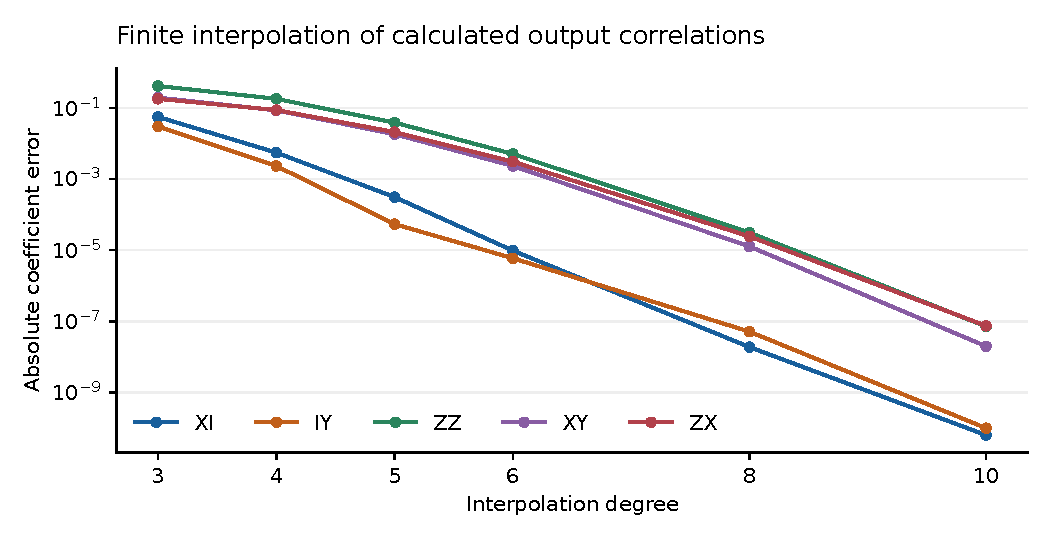
\includegraphics[width=.86\textwidth]{finite_derivative_convergence.pdf}
\caption{Executed finite interpolation of calculated ideal-instrument means.
This checks the new acquisition identity on a small model. It is not
experimental accuracy or an execution of the theorem's sampling budget.}
\end{figure}

The conservative theorem schedule was also evaluated. For
\(n=2,M=15,k=2,B_H=1.37,r=4,\kappa_0=2.46,\epsilon=0.1\), it gives
\[
T_0=4.58934,\qquad \eta=1.45264\times10^{-5},\qquad h=0.00667022.
\]
Two fully specified sufficient schedules were evaluated:
\begin{center}
\begin{tabular}{lrr}
\toprule Schedule & Degree & Total raw-trial upper bound\\ \midrule
Norm/Markov, separate nodal batches & \(52\)& \(10^{62.54}\)\\
Factorial tail, actual weights, randomized nodes & \(14\)& \(10^{39.12}\)\\
\bottomrule
\end{tabular}
\end{center}
The second evaluation inflates the calculated weight norm by a factor of
two, uses the finite dyadic-sampler concentration bound, and requires
timing accuracy about \(9.35\times10^{-24}\) in the model's time units.
It applies with the two-site complete neighborhoods, so no burn-in
is necessary. Both counts precede the continuous receiver compilation.
These are upper bounds, not lower bounds or proposed device settings.
It shows why a polynomial theorem alone does not establish a useful
laboratory or civilisation-scale consequence. No theorem-scale sampling,
protected factory or noisy field collector was simulated.

\section{Resource boundaries and preserved construction knowledge}
At source start \(I/d\), discard every purifier \(A\), retaining only P1's
mixed exports \(B\) and their flags. For each reset history, source and
fresh replacement baths are jointly maximally mixed, and every unitary
segment and wire exchange preserves that joint state. The full retained
\(B\) stream is therefore maximally mixed and independent of \(H\).
No collective measurement of this particular record can identify \(H\).
The positive operation uses additional actually delivered purifier
information. This is not an impossibility claim for every classical
measurement of the original fields.

If all payload information crosses an entanglement-breaking classical
record and later calibration contains no surviving quantum payload,
the final channel remains entanglement breaking. Its Choi overlap with
\(\Phi_d\) is at most \(1/d\), so its distance from identity is at least
\(2(1-1/d)\). The early quantum archive is substantive.

Stationarity is substantive too: later observations cannot identify an
arbitrary unobserved earlier drift. A changing Hamiltonian requires an
independently bounded discrepancy allowance. Missing terms outside the
candidate class, inaccessible source noise, unavailable purifiers and
unknown port gauges are not inferred away.

The previous construction package is preserved byte-for-byte as a
separate folder in the new source archive, including its complete
proofs, code, evidence and limits. In particular:
\begin{enumerate}
\item The full classical-feedback all-strength hidden-\(Z\) theorem keeps its
chronological full-CQ proof and per-branch budget. The sharper global-budget
theorem is separate; its constant is not extended to arbitrary branchwise feedback.
\item The matched fixed-order known-parity/GHZ law, finite-slew thresholds and
complete binary-POVM calibration remain. No general purity upper bound,
growing-order sharp theorem or zero-capacity conclusion is added.
\item The independent thermal-effusion operation retains its certified thin
barrier shell, actual force and clearing interface, finite angular quadrature,
flight/clearing/calibration costs and residual exposure
\(1/(\Gamma\Lambda_{\rm flux})\). It is not general natural-failure prediction.
\item P1's known-Hamiltonian reader and separate diagonal-in-one-product-basis
decoder keep their coherent-output and protected-memory premises.
\item P2's local unknown-support uncertainty construction stays within its
declared local reach, product invariant law and operating refresh backbone.
It does not certify arbitrary natural-system completeness.
\end{enumerate}

The achieved new consequence is a change in experimental ordering:
the first unknown state can be captured before its Hamiltonian is learned,
with reference-uniform recovery and a complete finite interface.
Practical efficiency and fixed physical hardware remain further requirements.

\begin{thebibliography}{99}
\bibitem{p1} Astra P1, \emph{Scalable output-only acquisition from interacting
many-body sources}, revision \texttt{324acb589443002bf8d529cc15e160129c5e36d2},
\url{https://github.com/harjassand/astra-research-knowledge/tree/324acb589443002bf8d529cc15e160129c5e36d2/research/returns/2026-11-05-p1-scalable-many-body-acquisition}.
\bibitem{p3} Astra P3, \emph{All-strength control speed}, same revision,
\url{https://github.com/harjassand/astra-research-knowledge/tree/324acb589443002bf8d529cc15e160129c5e36d2/research/returns/2026-11-05-p3-all-strength-control-speed}.
\bibitem{p2} Astra P2, \emph{Unknown local ports}, same revision,
\url{https://github.com/harjassand/astra-research-knowledge/tree/324acb589443002bf8d529cc15e160129c5e36d2/research/returns/2026-11-05-p2-unknown-local-ports}.
\bibitem{guta} M. Gu\c{t}\u{a} and J. Kiukas, \emph{Equivalence classes and local
asymptotic normality in system identification for quantum Markov chains},
Commun.\ Math.\ Phys.\ 335, 1397--1428 (2015),
\url{https://arxiv.org/abs/1402.3535}.
\bibitem{franca} D. Stilck Fran\c{c}a, L. A. Markovich, V. V. Dobrovitski,
A. H. Werner and J. Borregaard, \emph{Efficient and robust estimation of
many-qubit Hamiltonians}, Nature Communications 15, 311 (2024),
\url{https://doi.org/10.1038/s41467-023-44012-5}.
\bibitem{castaneda} J. Castaneda and N. Wiebe, \emph{Hamiltonian Learning via
Shadow Tomography of Pseudo-Choi States}, Quantum 9, 1700 (2025),
\url{https://arxiv.org/abs/2308.13020}.
\bibitem{haah} J. Haah, R. Kothari and E. Tang, \emph{Learning quantum
Hamiltonians from high-temperature Gibbs states and real-time evolutions},
Nature Physics 20, 1027--1031 (2024), \url{https://arxiv.org/abs/2108.04842}.
\bibitem{gong} W. Gong, M. Ma, S. Chen, J. Cotler and H.-Y. Huang,
\emph{Out-of-control Hamiltonian Learning}, arXiv:2610.06709
(5 October 2026), \url{https://arxiv.org/abs/2610.06709}.
\bibitem{liu} S. Liu, Z. Xu, A. V. Gorshkov, X. Wu, Y.-X. Wang and Z.-Y. Wei,
\emph{Learning Many-Body Hamiltonians Using a Local Probe}, arXiv:2610.02157
(1 October 2026), \url{https://arxiv.org/abs/2610.02157}.
\bibitem{navascues} M. Navascu\'es, \emph{Resetting Uncontrolled Quantum Systems},
Phys.\ Rev.\ X 8, 031008 (2018),
\url{https://doi.org/10.1103/PhysRevX.8.031008}.
\end{thebibliography}
\end{document}
